\documentclass[10pt]{article}
\usepackage[utf8]{inputenc}
\usepackage[T1]{fontenc}
\usepackage{amsmath}
\usepackage{amsfonts}
\usepackage{amssymb}
\usepackage[version=4]{mhchem}
\usepackage{stmaryrd}
\usepackage{bbold}
\usepackage{caption}
\usepackage{hyperref}
\hypersetup{colorlinks=true, linkcolor=blue, filecolor=magenta, urlcolor=cyan,}
\urlstyle{same}
\usepackage{graphicx}
\usepackage[export]{adjustbox}
\graphicspath{ {./images/} }

\title{Constructing Differentially 4 Uniform Permutations from Known Ones* }

\author{YU Yuyin ${ }^{1,2}$, WANG Mingsheng ${ }^{1,2}$ and LI Yongqiang ${ }^{1,2}$\\
(1.State Key Laboratory of Information Security, Institute of Information Engineering, Chinese Academy of Sciences, Beijing 100195, China)\\
(2.Graduate University of the Chinese Academy of Sciences, Beijing 100049, China)}
\date{}


%New command to display footnote whose markers will always be hidden
\let\svthefootnote\thefootnote
\newcommand\blfootnotetext[1]{%
  \let\thefootnote\relax\footnote{#1}%
  \addtocounter{footnote}{-1}%
  \let\thefootnote\svthefootnote%
}

%Overriding the \footnotetext command to hide the marker if its value is `0`
\let\svfootnotetext\footnotetext
\renewcommand\footnotetext[2][?]{%
  \if\relax#1\relax%
    \ifnum\value{footnote}=0\blfootnotetext{#2}\else\svfootnotetext{#2}\fi%
  \else%
    \if?#1\ifnum\value{footnote}=0\blfootnotetext{#2}\else\svfootnotetext{#2}\fi%
    \else\svfootnotetext[#1]{#2}\fi%
  \fi
}

\begin{document}
\maketitle
\captionsetup{singlelinecheck=false}


\begin{abstract}
Low differential uniformity functions provide good resistance to differential attacks. The AES (Advanced encryption standard) uses a differentially 4 uniform function (the inverse function) as its S -box. We give a further study of the inverse function in this paper. It is observed that after exchanging two values of a low differential uniformity function, its differential property still keeps good. Especially, for the inverse function over $\mathbb{F}_{2^{n}}$ ( $n$ even), various possible differential uniformities are completely determined after its two values are exchanged. As a consequence, we get some highly nonlinear permutations with differential uniformity 4 which are not CCZequivalent (Carlet Charpin-Zinoviev equivalent) to the inverse function on $\mathbb{F}_{2^{n}}$.
\end{abstract}

Key words - Block cipher, Advanced encryption standard (AES), S-box, Inverse function.

\section*{I. Introduction}
In today' s world where much of our personal information and financial transactions are processed via the Internet, data encryption is an essential element to any effective computer security system. This activity is why encryption is important. The block cipher AES (Advanced encryption standard) is the most famous encryption algorithm. The substitution box (in brief, S-box) provides confusion (a notion mentioned by C. Shannon) for the AES. Differential uniformity and nonlinearity are important parameters in the design of S-boxes. The AES uses a differentially 4 uniform function called the inverse function as its S-box. The inverse function has many very nice cryptographic properties. We give a further study of the inverse function in this paper. It is observed that after exchanging two values of the inverse function, its differential uniformity and nonlinearity still keep good. This result proves the robustness of the AES's S-box. We generalize it and give a new method to construct differentially 4 uniform functions with high nonlinearity.

We have introduced the background and motivation of our work, next we shall give some necessary definitions needed in the following.

The differential uniformity of a function can be defined as\\
follows:\\
Definition $1{ }^{[2]}$ Let $G_{1}$ and $G_{2}$ be finite Abelian groups. A mapping $F: G_{1} \rightarrow G_{2}$ is called differentially $\delta(F)$ uniform if

$$
\delta(F)=\max _{a \neq 0 \in G_{1}, b \in G_{2}} \# \Delta_{F}(a, b)
$$

where $\Delta_{F}(a, b)=\left\{x \in G_{1}: F(x+a)-F(x)=b\right\}, \# \Delta_{F}(a, b)$ is the cardinality of the set $\Delta_{F}(a, b)$. If $\delta(F)=2$, we can say that $F$ is APN (Almost perfect nonlinear).

We consider the differential property of the functions on the finite field $\mathbb{F}_{2^{n}}$. Note that APN functions provide optimal resistance to differential attack on $\mathbb{F}_{2^{n}}$. There has been much recent results on APN functions ${ }^{[3-9]}$ when $p=2$. However, at present we still don't know whether APN permutations exist on $\mathbb{F}_{2^{n}}$ ( $\mathbb{F}_{2^{n}}$ is the finite field with $2^{n}$ elements) with $n$ even and greater than 6. So the AES chooses the inverse function, which is differentially 4 uniform, as its S-box. As a matter of fact, even finding differentially 4 uniform permutation functions with high nonlinearity on even degree fields is a major challenge in cryptography.

The nonlinearity $n l(F)$ of a function on $\mathbb{F}_{2^{n}}$ is an indicator to measure the minimum distance between all the component functions of $F$ and all the affine functions. It quantifies the level of resistance of the S-box to the linear attack. We have:


\begin{equation*}
n l(F)=2^{n-1}-\frac{1}{2} \max _{a \neq 0, b \in \mathbb{F}_{2} n}\left|\lambda_{F}(a, b)\right| \tag{1}
\end{equation*}


where $\lambda_{F}(a, b)=\sum_{x \in \mathbb{F}_{2^{n}}}(-1)^{\operatorname{Tr}(a F(x)+b x)}$. We use Tr to denotes the absolute trace map from $\mathbb{F}_{2^{n}}$ to $\mathbb{F}_{2}$, that is, $\operatorname{Tr}(x)=\sum_{i=0}^{n-1} x^{2^{i}}$.

We introduce some differentially 4 uniform functions over $\mathbb{F}_{2^{n}}$ :

The inverse function defined on even degree field ${ }^{[2]}$, and it was used as the S-box of the AES when $n=8$.\\
(1) The Gold functions ${ }^{[10]} x^{2^{3}+1}$ with $n=2 k, k$ odd and $\operatorname{gcd}(n, s)=2$.\\
(2) The Kasami functions ${ }^{[11]} x^{2^{2 s}-2^{s}+1}$ with $n=2 k, k$ odd and $\operatorname{gcd}(n, s)=2$.\\
(3) The functions $x^{2^{2 k}+2^{k}+1}$ with $n=4 k, k$ odd $^{[5]}$.

\footnotetext{*Manuscript Received Apr. 2012; Accepted Sept. 2012. This work is supported by the National Natural Science Foundation of China (No.60970134, No.11171323, No.61173134), the IIE's Cryptography Research Project (No.Y2Z0011102), the Strategic Priority Research Program of the Chinese Academy of Sciences (No.XDA06010701).
}
(4) Carlet ${ }^{[7,12]}$ constructed a series of differentially 4 uniform functions.\\
(5) The new functions from exchanging two values of the APN function $F$ are differentially 4 uniform functions when they are not APN, as shown in this paper (see Proposition 1).\\
(6) The functions $I_{(0, v)}(x)$ (see Proposition 3) are differentially 4 uniform functions when $n=4 r+2(r \geq 1)$, and the functions $I_{(u, v)}(x)$ (see Theorem 1) are differentially 4 uniform functions when $n=2 m(m \geq 1), \operatorname{Tr}\left(u v^{-1}\right)=1$ and $\operatorname{Tr}\left(u^{-1} v\right)=1$, as shown in this paper.

An overwhelming majority cryptosystems were designed over $\mathbb{F}_{2^{2}}(t \geq 1)$. Therefore, finding differentially 4 uniform functions over $\mathbb{F}_{2^{2}}$ is especially useful. We can construct many new differentially 4 uniform functions over $\mathbb{F}_{2^{2}}$ with our method. Thus it is useful in practice.

Berger et al. ${ }^{[13]}$ investigated some open problems on APN functions over $\mathbb{F}_{2^{n}}$. As to the differentially 4 uniform permutations, they listed an open problem, which is equivalent to the following:

Problem 1 Find a permutation $F$ on $\mathbb{F}_{2^{n}}, n$ even, such that $\delta(F)=4$ and $A<2^{n}-1$, where $A=\#\{(a, b) \in \left.\mathbb{F}_{2^{n}} \times \mathbb{F}_{2^{n}} \mid \delta_{F}(a, b)=4, a \neq 0\right\}$.

In this paper, we find such permutations. We will give a detailed description on this result in Section II.

The paper is organized as follows. In Section II, we introduce some basic properties and applications of our method. In Section III, we give a detailed description on how to construct differentially 4 uniform from the inverse function.

\section*{II. Basic Properties and Applications}
\section*{1. Properties}
When we do a few changes on the values of a function, some properties of the function will not change too much. In this subsection, we will give a detailed description on such properties.

First, we introduce some useful lemmas.\\
Lemma $1{ }^{[14]}$ The equation $x^{2}+x+c=0$ has a solution in $\mathbb{F}_{2^{n}}$ if and only if $\operatorname{Tr}(c)=0$.

Lemma 2 Let $F, G$ be two functions from $\mathbb{F}_{2^{n}}$ into $\mathbb{F}_{2^{n}}$ such that:

$$
\begin{cases}G\left(p_{1}\right) \neq F\left(p_{1}\right), & p_{1} \in \mathbb{F}_{2^{n}} \\ G(x)=F(x), & x \in \mathbb{F}_{2^{n}} \text { and } x \neq p_{1}\end{cases}
$$

Then

$$
\begin{aligned}
& \delta(F)-2 \leq \delta(G) \leq \delta(F)+2, \text { and } \\
& n l(F)-1 \leq n l(G) \leq n l(F)+1
\end{aligned}
$$

Proof $F$ is different from $G$ only in one value. According to Definition 1, it is easy to see that for all $(a, b) \in\left(\mathbb{F}_{2^{n}}^{*} \times \mathbb{F}_{2^{n}}\right)$, there are

$$
\begin{aligned}
& \Delta_{F}(a, b) \subseteq \Delta_{G}(a, b) \cup\left\{p_{1}, p_{1}+a\right\}, \text { and } \\
& \Delta_{G}(a, b) \subseteq \Delta_{F}(a, b) \cup\left\{p_{1}, p_{1}+a\right\}
\end{aligned}
$$

which imply the first part of this proposition. Now let's consider the second part. For all $(a, b) \in\left(\mathbb{F}_{2^{n}}^{*} \times \mathbb{F}_{2^{n}}\right)$, let

$$
\lambda_{F}(a, b)=\sum_{x \in \mathbb{F}_{2^{n}}}(-1)^{\operatorname{Tr}(a F(x)+b x)}
$$

$$
\lambda_{G}(a, b)=\sum_{x \in \mathbb{F}_{2^{n}}}(-1)^{\operatorname{Tr}(a G(x)+b x)}
$$

By the definition of $G$, it can be deduced that


\begin{align*}
& \left|\lambda_{G}(a, b)-\lambda_{F}(a, b)\right| \\
& \quad=\left|(-1)^{\operatorname{Tr}\left(a G\left(p_{1}\right)+b p_{1}\right)}-(-1)^{\operatorname{Tr}\left(a F\left(p_{1}\right)+b p_{1}\right)}\right| \\
& \quad \leq 2 \tag{2}
\end{align*}


From Eqs.(1) and (2), we can get

$$
n l(F)-1 \leq n l(G) \leq n l(F)+1 .
$$

This proposition tells us that if we change only one value of a function, the differential and nonlinear properties of the function only change little, avalanche will not happen. This is really a good property which can be used to find new good functions from known ones. We will give some examples in the following subsection. First, we have a simple corollary of Lemma 2.

Corollary 1 Let $F$ be a function from $\mathbb{F}_{2^{n}}$ into $\mathbb{F}_{2^{n}}$. Define a new function $G$ as follows:

$$
G(x)= \begin{cases}F\left(p_{2}\right), & x=p_{1} \\ F\left(p_{1}\right), & x=p_{2}, p_{2} \neq p_{1} \\ F(x), & x \neq p_{1}, p_{2}\end{cases}
$$

Then for all $a \in \mathbb{F}_{2^{n}}^{*}, b \in \mathbb{F}_{2^{n}}$, there are $\Delta_{G}(a, b) \subseteq \Delta_{F}(a, b) \cup \left\{p_{1}, p_{1}+a, p_{2}, p_{2}+a\right\}$. Similar as in Lemma 2, there are

$$
\begin{aligned}
& \delta(F)-4 \leq \delta(G) \leq \delta(F)+4, \text { and } \\
& n l(F)-2 \leq n l(G) \leq n l(F)+2
\end{aligned}
$$

Especially, when $F$ is an APN function, we have the following result:

Proposition 1 Let $F$ and $G$ be the same as in Corollary 1. If $\delta(F)=2$, then

$$
\delta(G) \in\{2,4\} .
$$

Proof By Corollary 1, there is $2 \leq \delta(G) \leq 6$. We will prove $\delta(G) \neq 6$ in the following.

Assume that $\delta(G)=6$. Then for some $(a, b) \in \mathbb{F}_{2^{n}}^{*} \times \mathbb{F}_{2^{n}}$, there are $\Delta_{G}(a, b)=\left\{x_{1}, x_{1}+a, x_{2}, x_{2}+a, x_{3}, x_{3}+a\right\}$, and the elements in $\Delta_{G}(a, b)$ are different from each other. By Corollary 1, we have


\begin{equation*}
\Delta_{G}(a, b) \subseteq \Delta_{F}(a, b) \cup\left\{p_{1}, p_{1}+a, p_{2}, p_{2}+a\right\} \tag{3}
\end{equation*}


We know that $\delta_{F}(a, b)=2$ since $F$ is APN. Then there must be


\begin{equation*}
\left|\Delta_{G}(a, b) \cup\left\{p_{1}, p_{1}+a, p_{2}, p_{2}+a\right\}\right| \leq 6=\delta_{G}(a, b) \tag{4}
\end{equation*}


From Eqs.(3) and (4) we conclude that $\Delta_{G}(a, b)=\Delta_{F}(a, b) \cup \left\{p_{1}, p_{1}+a, p_{2}, p_{2}+a\right\}$, which implies $\left\{p_{1}, p_{1}+a, p_{2}, p_{2}+a\right\} \subseteq \Delta_{G}(a, b)$. So, without loss of generality, we can suppose that

$$
p_{1}=x_{1}, p_{2}=x_{2}
$$

Then we will have

$$
\left\{\begin{array}{l}
G\left(p_{1}+a\right)+G\left(p_{1}\right)=b \\
G\left(p_{2}+a\right)+G\left(p_{2}\right)=b
\end{array}\right.
$$

that is

$$
\left\{\begin{array}{l}
F\left(p_{1}+a\right)+F\left(p_{2}\right)=b \\
F\left(p_{2}+a\right)+F\left(p_{1}\right)=b
\end{array}\right.
$$

which is equal to

\[
\left\{\begin{array}{l}
F\left(p_{1}+a\right)+F\left(p_{1}+a+\left(a+p_{1}+p_{2}\right)\right)=b  \tag{5}\\
F\left(p_{2}+a\right)+F\left(p_{2}+a+\left(a+p_{1}+p_{2}\right)\right)=b
\end{array}\right.
\]

By Eq.(5), we deduce that the equation

$$
F(x)+F\left(x+\left(a+p_{1}+p_{2}\right)\right)=b
$$

has four solutions, which is impossible because $F$ is APN. So $\delta(G) \neq 6$, which implies the conclusion.

As a matter of fact, we never get differentially 2 uniform functions when we do tests in $\mathbb{F}_{2^{6}}$ and $\mathbb{F}_{2^{7}}$. The above transformation will keep its permutation property if the original function is a permutation.

\section*{2. Applications}
We have introduced an open problem proposed by Berger et al. in the introduction, here we give the details about what we have done to this problem. We specify this problem to $n=6$. First we introduce an APN permutation on $\mathbb{F}_{2^{6}}$ found by Dillon ${ }^{[8]}$, which is described by Table 1.

\begin{table}[h]
\begin{center}
\captionsetup{labelformat=empty}
\caption{Table 1. Value table of $F$}
\begin{tabular}{|c|c|c|c|c|c|c|c|}
\hline
0 & 54 & 48 & 13 & 15 & 18 & 53 & 35 \\
\hline
25 & 63 & 45 & 52 & 3 & 20 & 41 & 33 \\
\hline
59 & 36 & 2 & 34 & 10 & 8 & 57 & 37 \\
\hline
60 & 19 & 42 & 14 & 50 & 26 & 58 & 24 \\
\hline
39 & 27 & 21 & 17 & 16 & 29 & 1 & 62 \\
\hline
47 & 40 & 51 & 56 & 7 & 43 & 44 & 38 \\
\hline
31 & 11 & 4 & 28 & 61 & 46 & 5 & 49 \\
\hline
9 & 6 & 23 & 32 & 30 & 12 & 55 & 22 \\
\hline
\end{tabular}
\end{center}
\end{table}

We denote this function by $F$, which satisfies: $F(0)=0$, $F(1)=54, F(2)=48, \cdots, F(7)=35, F(8)=25, \cdots$, $F(63)=22$. According to Proposition 1, if we exchange $F(i)$ and $F(j)(i \neq j)$, then we get a lot of new functions, denoted as $F_{(i, j)}$, which satisfies $\delta\left(F_{(i, j)}\right) \in\{2,4\}$. It is plausible to expect that function $F_{(i, j)}$ will keep many properties of the original function $F$ (see Corollary 1). Based on these considerations, we traverse the pairs of $(i, j) \in\left(\mathbb{Z}_{2^{6}} \times \mathbb{Z}_{2^{6}}\right)(i \neq j)$, and finally find some $A<2^{6}-1$, which satisfies the requirements of Problem 1. We give an example as follows:

Example 1 Exchanging values of $F(0)$ and $F(1)$ to get a new function $F_{(0,1)}$. Easy to compute that $\delta\left(F_{(0,1)}\right)=4$, and the corresponding parameter $A=54<2^{6}-1$. Thus we have found an example of Problem 1.

In fact, 1176 examples are found when we traverse the pairs of $(i, j) \in\left(\mathbb{Z}_{2^{6}} \times \mathbb{Z}_{2^{6}}\right)$, where $i<j$.

\section*{III. Constructing Differentially 4 Uniform Permutations from the Inverse Function}
In this section, we will give a detailed discussion about the inverse function with the above idea. First we recall a formal definition about the inverse function.

Definition 2 Define the inverse function $I$ on $\mathbb{F}_{2^{n}}$ as follows:

$$
I(x)= \begin{cases}0, & x=0 \\ x^{-1}, & x \neq 0\end{cases}
$$

Let $0^{-1}=0$, and we only consider the case when $n=2 m$ in the rest of this section.

It is well known that $\delta(I)=4$ when $n$ is even ${ }^{[2]}$, we restate this result as follows:

Lemma 3 Let $d=\frac{1}{3}\left(2^{2 m}-1\right)(m \geq 1)$, and $g$ a primitive element in $\mathbb{F}_{2^{2 m}},(a, b) \in \mathbb{F}_{2^{2 m}}^{*} \times \mathbb{F}_{2^{2 m}}$ Then the following statements are equivalent:\\
(1) $\delta_{I}(a, b)=4$;\\
(2) $b=a^{-1}$;\\
(3) $\Delta_{I}(a, b)=\left\{0, a, a g^{d}, a g^{2 d}\right\}$.

Proposition 2 Let $u, v \in \mathbb{F}_{2^{2 m}}$ with $u \neq v$. Define a new function $I_{(u, v)}(x)$ on $\mathbb{F}_{2^{2 m}}(m \geq 1)$ as follows:

$$
I_{(u, v)}(x)= \begin{cases}I(v), & x=u \\ I(u), & x=v, v \neq u \\ I(x), & x \neq u, v\end{cases}
$$

Then for all $\left.(u, v) \in\left(\mathbb{F}_{2^{2 m}} \times \mathbb{F}_{2^{2 m}}\right) u \neq v\right)$, we have

$$
\delta\left(I_{(u, v)}\right) \leq 6
$$

Proof By Corollary 1, there is $\delta\left(I_{(u, v)}\right) \leq 8$. Suppose $\delta\left(I_{(u, v)}\right)=8$. From Corollary 1 and Lemma 3, we know that this happens only when $\Delta_{I_{(u, v)}}(a, b)=\left\{0, a, a g^{d}, a g^{2 d}, u, u+\right. a, v, v+a\}$ for some $a, b \in \mathbb{F}_{2^{2 m}}, b=a^{-1}(a \neq 0)$, and the eight elements in $\Delta_{I_{(u, v)}}(a, b)$ are pairwise different. It is easy to see that $u(u+a) v(v+a) \neq 0$ (If not, there must be repeated elements in $\left.\Delta_{I_{(u, v)}}(a, b)\right)$. Thus we have

$$
\left\{\begin{array}{l}
I_{(u, v)}(u)+I_{(u, v)}(u+a)=a^{-1} \\
I_{(u, v)}(v)+I_{(u, v)}(v+a)=a^{-1}
\end{array}\right.
$$

which is equivalent to

$$
\left\{\begin{array}{l}
v^{-1}+(u+a)^{-1}=a^{-1} \\
u^{-1}+(v+a)^{-1}=a^{-1}
\end{array}\right.
$$

From the above equations we can get

$$
\left\{\begin{array}{l}
u a=a^{2}+u v \\
v a=a^{2}+u v
\end{array}\right.
$$

So we can deduce that $v a=u a$, which implies $u=v$ (Note that $a \neq 0$ ). This result contradicts with the premise that $u \neq v$. So $\delta\left(I_{(u, v)}\right)$ cannot reach the upper bound given in Corollary 1, thus $\delta\left(I_{(u, v)}\right) \leq 6$.

Proposition 3 Let $I_{(u, v)}$ be the function defined in Proposition 2, suppose $u=0$ and $v \neq 0$, then we have


\begin{equation*}
I_{(0, v)}(x)=(x+v)^{-1}+v\left(x^{2}+v x\right)^{-1} \tag{6}
\end{equation*}


and

\[
\begin{cases}\delta\left(I_{(0, v)}\right)=6, & \text { iff } m=2 r  \tag{7}\\ \delta\left(I_{(0, v)}\right) \leq 4, & \text { iff } m=2 r+1, r \geq 1\end{cases}
\]

Proof By Proposition 2, we only need to prove the first part of Eq.(7). Let $F(x)=(x+v)^{-1}+v\left(x^{2}+v x\right)^{-1}$. It is easy to check that

$$
\left\{\begin{array}{l}
F(0)=v^{-1}=I(v) \\
F(v)=0=I(0) \\
F(x)=x^{-1}=I(x), \quad x \neq 0, v
\end{array}\right.
$$

So Eq.(6) follows.\\
For any $a \in \mathbb{F}_{2^{2 m}}^{*}, b \in \mathbb{F}_{2^{2 m}}$, equation $F(x)+F(x+a)=b$ becomes


\begin{equation*}
(x+v)^{-1}+v\left(x^{2}+v x\right)^{-1}+(x+v+a)^{-1}+v\left(x^{2}+v x+a^{2}+v a\right)^{-1}=b \tag{8}
\end{equation*}


When $a=v$, Eq.(8) becomes $x^{-1}+(x+v)^{-1}=b$, which has at most 4 roots. Then we suppose $a \neq v$. First, it is easy to see that $v$ is a root of Eq.(8) if and only if

$$
b=a^{-1}+v\left(a^{2}+v a\right)^{-1}=(a+v)^{-1}
$$

and 0 is a root of Eq.(8) if and only if

$$
b=v^{-1}+(v+a)^{-1}+v\left(a^{2}+v a\right)^{-1}=v^{-1}+a^{-1}
$$

Therefore, we have the following cases:\\
Case $1 \quad b=(a+v)^{-1}$ and $b \neq v^{-1}+a^{-1}$. This means $v$ is a root of Eq.(8) but 0 is not. Notice that, since $F(x)=x^{-1}$ when $x \neq 0, v$, the existence of $x_{0} \in \mathbb{F}_{2^{2 m}}\{0, a, v, v+a\}$ satisfying Eq.(8) implies

$$
b=F\left(x_{0}\right)+F\left(x_{0}+a\right)=x_{0}^{-1}+\left(x_{0}+a\right)^{-1}
$$

which has at most two more roots. Therefore, Eq.(8) has at most 4 roots in this case.

Case $2 \quad b=v^{-1}+a^{-1}$ and $b \neq(a+v)^{-1}$. Similar as in Case 1, Eq.(8) has at most 4 roots in this case.

Case $3 b=(a+v)^{-1}=v^{-1}+a^{-1}$, which means both 0 and $v$ are the roots of Eq.(8). The equation $(a+v)^{-1}= v^{-1}+a^{-1}$ is equivalent to $\left(\frac{a}{v}\right)^{2}+\frac{a}{v}+1=0$, which implies $\left(\frac{a}{v}\right)^{3}=1$, i.e. $\left(\frac{a}{v}\right)^{-2}=\frac{a}{v}$. Similar as Case 1, the existence of $x_{0} \in \mathbb{F}_{2^{2 m}} \backslash\{0, a, v, v+a\}$ satisfying Eq.(8) implies $x_{0}^{-1}+\left(x_{0}+a\right)^{-1}=v^{-1}+a^{-1}$, which is equivalent to

$$
\left(\frac{x_{0}}{a}\right)^{2}+\frac{x_{0}}{a}=\left(\frac{a}{v}+1\right)^{-1}=\left(\frac{a}{v}\right)^{-2}=\frac{a}{v}
$$

According to Lemma 1, the above equation is true if and only $\operatorname{Tr}\left(\frac{a}{v}\right)=0$. Therefore, Eq.(8) has six roots if and only if $m$ is even, since

$$
\begin{aligned}
\operatorname{Tr}\left(\frac{a}{v}\right) & =\sum_{i=0}^{2 m-1}\left(\frac{a}{v}\right)^{2^{i}} \\
& =\sum_{j=0}^{m-1}\left(\left(\frac{a}{v}\right)^{2^{2 j}}+\left(\frac{a}{v}\right)^{2^{2 j+1}}\right) \\
& =m \bmod 2
\end{aligned}
$$

It is easy to check that the six roots $0, a, v, v+a, x_{0}, x_{0}+a$ are pairwise different since

$$
\left(\frac{x_{0}}{a}\right)^{2}+\frac{x_{0}}{a}=\frac{a}{v} \neq 1
$$

Case $4 \quad b \neq(a+v)^{-1}, b \neq v^{-1}+a^{-1}$. This means neither 0 or $v$ is a root of Eq.(8). Similar as in Case 1, Eq.(8) has at most 4 roots in this case.

Remark 1 Simple computation shows that when $m=4$, $n l\left(I_{(0, v)}\right)=112$; when $m=3, n l\left(I_{(0, v)}\right)=24$, which is the same as the inverse function.

Until now, we have introduced some special cases about the transformations of the inverse function $I(x)$. Together with the following theorem we will have a comprehensive understanding about the differential character of all these transformation functions.

Theorem 1 Let $I_{(u, v)}$ be defined as in Proposition 2, then for all $u, v \in \mathbb{F}_{2^{2 m}}$ with $u \neq v$ and $u v \neq 0$, we have:


\begin{equation*}
\delta\left(I_{(u, v)}\right)=6, \text { iff } \operatorname{Tr}\left(u v^{-1}\right)=0 \text { or } \operatorname{Tr}\left(u^{-1} v\right)=0 \tag{9}
\end{equation*}


and


\begin{equation*}
\delta\left(I_{(u, v)}\right)=4, \text { iff } \operatorname{Tr}\left(u v^{-1}\right)=\operatorname{Tr}\left(u^{-1} v\right)=1 \tag{10}
\end{equation*}


Proof Let $F(x)=I_{(u, v)}(x), d=\frac{1}{3}\left(2^{2 m}-1\right)$, and $g$ be a primitive element in $\mathbb{F}_{2^{2 m}}$. We want to investigate roots of the equation


\begin{equation*}
F(x)+F(x+a)=b \tag{11}
\end{equation*}


For $a \in \mathbb{F}_{2^{2 m}}^{*}, b \in \mathbb{F}_{2^{2 m}}$. First, suppose $a=u+v$, then we have the following cases:

Case 1.1 $u$ is a root of Eq.(11). Therefore, $v=u+a$ also satisfies Eq.(11) and $b=u^{-1}+v^{-1}$. If there exists $x_{0} \in \mathbb{F}_{2^{2 m}} \backslash\{u, v\}$ which satisfies Eq.(11), then


\begin{equation*}
b=F\left(x_{0}\right)+F\left(x_{0}+a\right)=x_{0}^{-1}+\left(x_{0}+a\right)^{-1} \tag{12}
\end{equation*}


When $a \neq b^{-1}$, it has at most two roots and Eq.(11) has at most 4 roots. When $u^{-1}+v^{-1}=b=a^{-1}=(u+v)^{-1}$, which happens if and only if $\left(\frac{u}{v}\right)^{2}+\frac{u}{v}=1$, it is obvious that the four roots of $x^{-1}+(x+u+v)^{-1}=(u+v)^{-1}$ are $0, u+v, v, u$. Thus Eq.(11) has at most 4 roots in this case.

Case $1.2 \quad u$ is not a root of Eq.(11). Therefore, $v$ is not a root of Eq.(11) either. Then if there exists $x_{0}$ which satisfies Eq.(11), it also satisfies Eq.(12), which has at most 4 roots.

Next, we suppose $a \neq u+v$. Notice that $u$ is a root of Eq.(11) if and only if\\
$b=F(u)+F(u+a)=v^{-1}+(u+a)^{-1}$ since $u+a \neq u, v$. Similarly, $v$ is a root of Eq.(11) if and only if

$$
b=u^{-1}+(v+a)^{-1}
$$

Then we have the following cases:\\
Case $2.1 \quad b=v^{-1}+(u+a)^{-1}=u^{-1}+(v+a)^{-1}$. This means that both $u$ and $v$ are roots of Eq.(11). Notice that $v^{-1}+(u+a)^{-1}=u^{-1}+(v+a)^{-1}$ is equivalent to $a=u$ or $v$ and $u^{2}+v^{2}+u v=0$. Otherwise, $v^{-1}+(u+a)^{-1}=u^{-1}+(v+a)^{-1}$ implies $u^{2}+v^{2}=a(u+v)$, which can not happen since $u \neq v$ and $a \neq u+v$. First, if $a=u$ and $u^{2}+v^{2}+u v=0$, then $0, u, v, v+u$ satisfy Eq.(11). As in Case 1.1, the existence of $x_{0} \in \mathbb{F}_{2^{n}} \backslash\{0, u, v, v+u\}$ satisfying Eq.(11) implies

$$
x_{0}^{-1}+\left(x_{0}+u\right)^{-1}=v^{-1}
$$

which is equivalent to $\left(\frac{x_{0}}{u}\right)^{2}+\frac{x_{0}}{u}=\frac{v}{u}$. Thus it has extra two more roots $x_{0}, x_{0}+u$ if and only if $\operatorname{Tr}\left(\frac{v}{u}\right)=0$. It is easy to check that $0, u, v, v+u, x_{0}, x_{0}+u$, which are the six roots of Eq.(11), are pairwise different since $u \neq v$ and $\left(\frac{x_{0}}{u}\right)^{2}+\frac{x_{0}}{u}=\frac{v}{u}$.

Similarly, if $a=v$ and $u^{2}+v^{2}+u v=0$, then Eq.(11) has six roots if and only if $\operatorname{Tr}\left(\frac{u}{v}\right)=0$.

Case $2.2 b=v^{-1}+(u+a)^{-1}$ and $b \neq u^{-1}+(v+a)^{-1}$. This means that $u$ is a root of Eq.(11) but $v$ is not. As in Case 1.1, the existence of $x_{0} \in \mathbb{F}_{2^{n}} \backslash\{u, u+a, v, v+a\}$ satisfying Eq.(11) implies

$$
x_{0}^{-1}+\left(x_{0}+a\right)^{-1}=v^{-1}+(u+a)^{-1}
$$

It has four roots if and only if $v^{-1}+(u+a)^{-1}=a^{-1}$. Notice that $a \neq u$ or $v$ since $u \neq v$, then it is equivalent to

$$
\left(\frac{a}{u}\right)^{2}+\frac{a}{u}=\frac{v}{u}
$$

Thus Eq.(11) has six roots if and only if $\operatorname{Tr}\left(\frac{v}{u}\right)=0$. Similar as in Case 2.1, we can check that $0, a, a g^{d}, a g^{2 d}, u, u+a$,\\
which are the six roots of Eq.(11) (see Lemma 3), are pairwise different. Also note that such $a$ satisfies the premise $b=v^{-1}+(u+a)^{-1} \neq u^{-1}+(v+a)^{-1}$, since $a \neq u$ or $v$.

Case $2.3 b=u^{-1}+(v+a)^{-1}$ and $b \neq v^{-1}+(u+a)^{-1}$. This means $v$ is a root of Eq.(11) but $u$ is not. Similar as Case 2.2, Eq.(11) has six roots if and only if $\operatorname{Tr}\left(\frac{u}{v}\right)=0$.

Case $2.4 \quad b \neq v^{-1}+(u+a)^{-1}$ and $u^{-1}+(v+a)^{-1}$. Then the roots of Eq.(11) are also the roots of Eq.(12), which has at most four roots.

Therefore, the number of roots of Eq.(11) is less than or equal to 4 if and only if $\operatorname{Tr}\left(\frac{u}{v}\right)=\operatorname{Tr}\left(\frac{v}{u}\right)=1$. Then we complete the proof.

Let $L_{1}$ and $L_{2}$ be two affine transformations on $\mathbb{F}_{2^{n}}$. For a function $F$ on $\mathbb{F}_{2^{n}}$, it is easy to check that $\left(L_{2} \circ F \circ L_{1}\right)_{(u, v)}= L_{2} \circ F_{\left(L_{1}(u), L_{1}(v)\right)} \circ L_{1}$ when $L_{1}$ is a permutation and $u, v \in \mathbb{F}_{2^{n}}$. Thus the following Corollary follows from Theorem 1.

Corollary 2 Let $L_{1}$ and $L_{2}$ be two affine transformations on $\mathbb{F}_{2^{2 m}}$ and $L_{1}$ is a permutation. $u, v \in \mathbb{F}_{2^{2 m}}$ such that $L_{1}(u) \neq 0$ and $L_{1}(v) \neq 0$. Then $\left(L_{2} \circ I \circ L_{1}\right)_{(u, v)}$ is differentially 4 uniform if and only if $\operatorname{Tr}\left(L_{1}(u) L_{1}(v)^{-1}\right)= \operatorname{Tr}\left(L_{1}(u)^{-1} L_{1}(v)\right)=1$.

Remark 2 When $m=4$, all the 32385 different functions support this theorem. There are 9180 functions with differentially 4 uniform property, and the 32385 functions have the same nonlinearity 110, so all the new constructed functions are not CCZ-equivalent to the original inverse function $I(x)$, which has the nonlinearity 112 . It can be seen that we really construct some new functions with this method, but we should also note that there are many equivalence relations in the new functions. We also get polynomial form of all the 32385 functions, according to our observation, each polynomial has more than 230 nonzero coefficients, all these polynomials are very complex. For example, we use the primitive polynomial $x^{8}+x^{4}+x^{3}+x^{2}+1$ to construct the finite field $\mathbb{F}_{2^{8}}, g$ is a root of $x^{8}+x^{4}+x^{3}+x^{2}+1=0$, choosing the function $I_{\left(g^{1}, g^{12}\right)}$, it is easy to check that $n l\left(I_{\left(g^{1}, g^{12}\right)}\right)=110$, $\delta\left(I_{\left(g^{1}, g^{12}\right)}\right)=4$, and $A=477$ (The definition of $A$ can be found in Problem 1). As for $I(x)$, it is well known that $n l(I)=112$, $\delta(I)=4$, the corresponding parameter $A=255$.

\section*{V.Conclusion}
We proposed a method for constructing differentially 4 uniform permutations and proved some properties of it in this paper. With this method we partly solved an open problem proposed by Berger et al. ${ }^{[13]}$ and constructed some new differentially 4 uniform functions with high nonlinearity in the even degree fields, which might be useful in the design of cryptographic algorithms.

\section*{References}
[1] C. Carlet, P. Charpin and V. Zinoviev, "Codes, bent functions and permutations suitable for DES-like cryptosystems", Designs, Codes and Cryptography, Vol.15, No.2, pp.125-156. 1998.\\[0pt]
[2] K. Nyberg, "Differentially uniform mappings for cryptography", Proceedings of EUROCRYPT'93, LNCS 765, pp.55-64, 1994.\\[0pt]
[3] L. Budaghyan, C. Carlet and G. Leander, "Constructing new APN functions from known ones", Finite Fields and Their Ap-\\
plications, Vol.15, No.2, pp.150-159, 2009.\\[0pt]
[4] L. Budaghyan, C. Carlet, G. Leander, "Two classes of quadratic APN binomials inequivalent to power functions", IEEE Trans. Inform. Theory, Vol.54, No.9, pp.4218-4229, 2008.\\[0pt]
[5] C. Bracken, G. Leander, "A highly nonlinear differentially 4 uniform power mapping that permutes fields of even degree", Finite Fields and Their Applications, Vol.16, No.4, pp.231-242, 2010.\\[0pt]
[6] K. Browning, J.F. Dillon, R.E. Kibler and M. McQuistan, "APN polynomials and related codes", Special volume of Journal of Combinatorics, Information and System Sciences, honoring the 75-th birthday of Prof. D.K. Ray-Chaudhuri, Vol.34, No.1-4, pp.135-159, 2009.\\[0pt]
[7] C. Carlet, "Relating three nonlinearity parameters of vectorial functions and building APN functions from bent functions", Designs, Codes and Cryptography, Vol.59, No.1-3, pp.89-109, 2011.\\[0pt]
[8] J.F. Dillon, "APN polynomials: an update (ppt)", Fq9, The 9th International Conference on Finite Fields and Applications, Dublin, Ireland, 2009.\\[0pt]
[9] Y. Edel, A. Pott, "A new almost perfect nonlinear function which is not quadratic", Adv. Math. Commun., Vol.3, pp.5981, 2009.\\[0pt]
[10] R. Gold, "Maximal recursive sequences with 3 -valued recursive cross-correlation functions", IEEE Trans. Inform. Theory, Vol.14, No.1, pp.154-156, 1968.\\[0pt]
[11] T. Kasami, "The weight enumerators for several classes of subcodes of the second order binary Reed-Muller codes", Inform. Control, Vol.18, pp.369-394, 1971.\\[0pt]
[12] C. Carlet, "On known and new differentially uniform functions", ACISP 2011, LNCS 6812, Springer-Verlag Berlin Heidelberg, pp.1-15, 2011.\\[0pt]
[13] T.P. Berger, A. Canteaut, P. Charpin and Y. Laigle-Chapuy, "On almost perfect nonlinear functions over $\mathbb{F}_{2^{n}}$ ", IEEE Trans. Inform. Theory, Vol.52, No.9, pp.4160-4170, 2006.\\[0pt]
[14] R. Lidl, H. Niederreiter, Finite Fields, Cambridge, U.K.: Cambridge Univ. Press, pp.56, 1983. \href{mailto:yongq.lee@gmail.com}{yongq.lee@gmail.com})\\
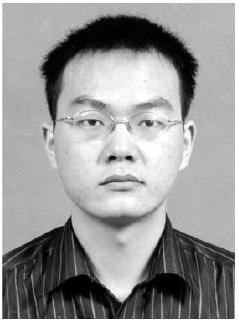
\includegraphics[max width=\textwidth, alt={}, center]{7f75cd8d-10b3-4472-8f4c-0cdd1ff17d74-5_325_239_1465_1121}\\
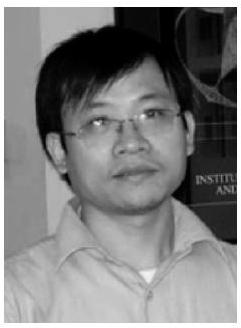
\includegraphics[max width=\textwidth, alt={}, center]{7f75cd8d-10b3-4472-8f4c-0cdd1ff17d74-5_328_241_1791_1119}

WANG Mingsheng received the Ph.D. degree in 1994 from Beijing Normal University, Beijing, China. At present he is a research professor at Institute of Information Engineering, Chinese Academy of Sciences, Beijing. His research interests lie in computational algebra, cryptography, and information security. (Email: \href{mailto:mswang@yahoo.cn}{mswang@yahoo.cn})

LI Yongqiang received the B.S. and M.S. degrees in mathematics from Beijing Normal University, Beijing, China, in 2005 and 2008 respectively, and the Ph.D. degree in information security from Institute of Software, Chinese Academy of Sciences, China, in January 2012. At present he is an assistant professor at Institute of Information Engineering, Chinese Academy of Sciences. His research interests lie in

YU Yuyin received the B.S. degree in computer science from Henan Normal University, Henan, China. At present, he is a Ph.D. candidate at Institute of Infomation Engineering, Chinese Academy of Sciences, Beijing. His research interests include APN functions, cryptographic algorithms and related areas. (Email: \href{mailto:yuyuyin@163.com}{yuyuyin@163.com})

WANG Mingsheng received the\\
D. degree in 1994 from Beijing Normal\\
aversity, Beijing, China. At present he\\
research professor at Institute of In-\\
mation Engineering, Chinese Academy\\
Sciences, Beijing. His research inter-\\
s lie in computational algebra, cryptog-\\
hy, and information security. (Email:\\
\href{mailto:wang@yahoo.cn}{wang@yahoo.cn})\\
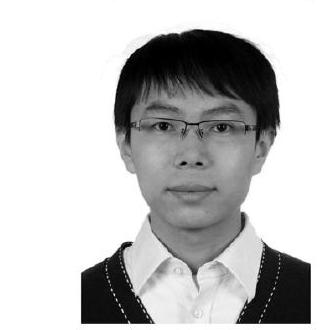
\includegraphics[max width=\textwidth, alt={}, center]{7f75cd8d-10b3-4472-8f4c-0cdd1ff17d74-5_330_321_2118_1044}\\
cryptography and related areas. (Email:


\end{document}